\documentclass{article}
\usepackage{graphicx}
\usepackage{amsmath}
\usepackage{tikz}
\usepackage[all]{xy}
\usetikzlibrary{positioning,chains,fit,shapes,calc}

\begin{document}

\title{Homework 1}
\author{Josh Cai}

\maketitle
\section*{Section 9.1}



\textbf{2a)} R = \{(1,1),(1,2),(1,3),(1,4),(1,5),(1,6),(2,2),(2,4),(2,6),(3,3),(3,6),(4,4),(5,5),(6,6)\}
\\\\
\textbf{2b)} 
\\
\definecolor{black}{RGB}{0,0,0}
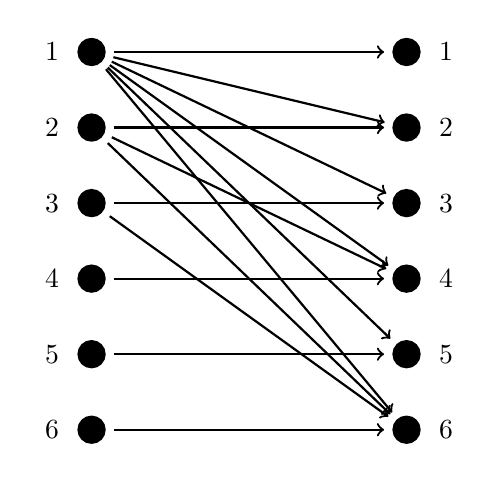
\begin{tikzpicture}[thick,
  every node/.style={draw,circle},
  fsnode/.style={fill=black},
  ssnode/.style={fill=black},
  every fit/.style={ellipse,draw,inner sep=-2pt,text width=2cm},
  ->,shorten >= 3pt,shorten <= 3pt
]
\begin{scope}[start chain=going below,node distance=6mm]
\foreach \i in {1,2,...,6}
  \node[fsnode,on chain] (f\i) [label=left: \i] {};
\end{scope}
\begin{scope}[xshift=4cm,start chain=going below,node distance=6mm]
\foreach \i in {1,2,...,6}
  \node[ssnode,on chain] (s\i) [label=right: \i] {};
\end{scope}
\draw (f1) -- (s1);
\draw (f1) -- (s2);
\draw (f1) -- (s3);
\draw (f1) -- (s4);
\draw (f1) -- (s5);
\draw (f1) -- (s6);
\draw (f2) -- (s2);
\draw (f2) -- (s4);
\draw (f2) -- (s6);
\draw (f3) -- (s3);
\draw (f3) -- (s6);
\draw (f4) -- (s4);
\draw (f5) -- (s5);
\draw (f6) -- (s6);
\end{tikzpicture}

\\\\

\textbf{2c)}
\begin{tabular}{ c | c c c c c c }
  R & 1 & 2 & 3 & 4 & 5 & 6 \\ \hline
  1 & X & X & X & X & X & X \\ 
  2 & 0 & X & 0 & X & 0 & X \\
  3 & 0 & 0 & X & 0 & 0 & X \\ 
  4 & 0 & 0 & 0 & X & 0 & 0 \\ 
  5 & 0 & 0 & 0 & 0 & X & 0 \\ 
  6 & 0 & 0 & 0 & 0 & 0 & X \\ 
\end{tabular}
\\\\
\textbf{26a)} $R^{-1}=\{(b,a)|a<b\}$
\\\\
\textbf{26b)} $\overline{R}=\{(a,b)|a\ge b\}$
\\\\
\textbf{28a)} $R^{-1}=\{(b,a)|a$ borders $b\}$
\\\\
\textbf{28b)} $\overline{R}=\{(a,b)|a$ doesn't border $b\}$
\\\\
\textbf{42} \{\}
\\\{(0,0)\}
\\\{(0,1)\}
\\\{(1,0)\}
\\\{(1,1)\}
\\\{(0,0), (0,1)\}
\\\{(0,0), (1,0)\}
\\\{(0,0), (1,1)\}
\\\{(0,1), (1,0)\}
\\\{(0,1),(1,1)\}
\\\{(1,0), (1,1)\}
\\\{(0,0), (0,1), (1,0)\}
\\\{(0,0), (0,1),(1,1)\}
\\\{(0,0), (1,0), (1,1)\}
\\\{(0,1), (1,0), (1,1)\}
\\\{(0,0), (0,1), (1,0), (1,1)\}
\\\\
\textbf{Additional} 8 relations, \{\{(1,1)\},\{(0,0), (1,1)\},\{(0,1),(1,1)\},\{(1,0), (1,1)\},\{(0,0), (0,1),(1,1)\},\{(0,0), (1,0), (1,1)\},\{(0,1), (1,0), (1,1)\},\{(0,0), (0,1), (1,0), (1,1)\}\}

\section*{Section 9.2}
\textbf{2)} \{(6,1,1,1),
(1,6,1,1),
(1,1,6,1),
(1,1,1,6),
(2,3,1,1),
(2,1,3,1),
(2,1,1,3),
(1,2,3,1),
(1,2,1,3),
(1,1,2,3),
(3,2,1,1),
(3,1,2,1),
(3,1,1,2),
(1,3,2,1),
(1,3,1,2),
(1,1,3,2)\}


\section*{Section 9.3}
\textbf{2a)}
\[
 \begin{bmatrix}
  0 & 1 & 1 & 1\\
  0 & 0 & 1 & 1\\
  0 & 0 & 0 & 1\\
  0 & 0 & 0 & 0
 \end{bmatrix}
\]
\\\\
\textbf{2b)}
\[
 \begin{bmatrix}
  1 & 0 & 0 & 1\\
  0 & 1 & 0 & 0\\
  0 & 0 & 1 & 0\\
  1 & 0 & 0 & 0
 \end{bmatrix}
\]
\\\\
\textbf{2c)}
\[
 \begin{bmatrix}
  0 & 1 & 1 & 1\\
  1 & 0 & 1 & 1\\
  1 & 1 & 0 & 1\\
  1 & 1 & 1 & 0
 \end{bmatrix}
\]
\\\\
\textbf{2d)}
\[
 \begin{bmatrix}
  0 & 0 & 0 & 0\\
  0 & 0 & 0 & 1\\
  1 & 1 & 0 & 1\\
  0 & 0 & 0 & 0
 \end{bmatrix}
\]
\\\\
\textbf{4a)}\{(1,1),(1,2),(1,4),(2,1),(2,3),(3,2),(3,3),(3,4),(4,1),(4,3),(4,4)\}
\\\\
\textbf{4b)}\{(1,1),(1,2),(1,3),(2,2),(3,3),(3,4),(4,1),(4,4)\}
\\\\
\textbf{4c)}\{(1,2),(1,4),(2,1),(2,3),(3,2),(3,4),(4,1),(4,3)\}
\\\\
\textbf{12)} $R^{-1}$ is the transposition of the matrix R. ($[A^{T}]_{ij}=[A]_{ji}$)
\\\\
\textbf{20)}
\begin{displaymath}
    \xymatrix{1 \ar@/^/[d]\ar@(dl,ul) & 2\ar@(dl,ul) \\
              3 \ar@/^/[u]\ar@(dl,ul) }
\end{displaymath}

\begin{displaymath}
    \xymatrix{1 \ar[r] & 2\ar@(dr,ur) \\
              3 \ar[ur] }
\end{displaymath}
\begin{displaymath}
    \xymatrix{1 \ar@/^/[d]\ar@/^/[r]\ar@(dl,ul) & 2\ar@/^/[dl] \ar@/^/[l] \\
              3 \ar@/^/[u]\ar@/^/[ur]\ar@(dl,ul) }

\end{displaymath}
\textbf{22)}
\begin{displaymath}
    \xymatrix{a \ar[r] \ar@(dl,ul) & b\ar@/^/[dl] \\
              c \ar[r]\ar@/^/[ur] & d\ar[ul]\ar[u] }

\end{displaymath}

\textbf{24)}\{(a,a),(a,c),(c,c),(b,c),(b,a),(b,b)\}
\\\\
\textbf{26)}\{(a,a),(a,b),(c,c),(c,a),(c,d),(b,a),(b,b),(d,d)\}
\\\\
\textbf{34)} Take the complete directed graph and erase all edges that are present in R to find $\overline{R}$.
\\\\





























\end{document}